\section{Protocol Design}

\subsection{Protocol Overview}

\begin{figure}[!h]
    \begin{center}
        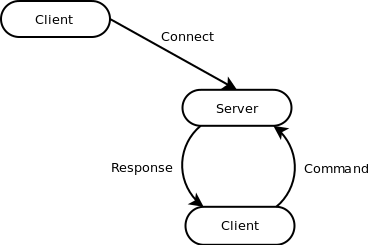
\includegraphics[scale=0.65]{chapter2/diagrams/protocol_high_level.png}
        \caption{The exchange of messages between a client and the server}
        \label{highLevelDia}
    \end{center}
\end{figure}

Gim uses a client-server architecture, where one computer (known as the Sever) acts as a central point which other computers (the Clients) connect. The clients do no communicate directly with each other and all communication takes place between the clients and the server. If a client wishes to send a message to another client it must first got through the server.

In GIM, the Protocol is responsible for enabling communication between the clients and the server in a reliable and consistent manner. A protocol is a set of rules that determine the format and transmission of data between computers. The syntax (the structure, or format) and semantics (the meaning) of the Protocol are discussed in the next section.

At the highest level of abstraction, the GIM Protocol works in a very simple manner.  A client connects to the sever and they exchange messages until the connection is closed, as shown in Figure ~\ref{highLevelDia}.

In practice there are several clients connected to the server at once, however as the clients do not directly interact with each other and do not need to know about each other, the entire system can be simplified as described above.



\subsection{Protocol Specification}

\subsection{Protocol Evolution}
